\section{C++}


\begin{frame}{Was ist C++?}
	\begin{block}{Eine standardisierte Programmiersprache}
		C++
		\begin{itemize}
			\item ist eine Programmiersprache (gibt einen Programmablauf vor)
			\item vereint sowohl high-level- wir auch low-level-Features
			\item ist sehr hardwarenah
			\item ist standardisiert (\emph{hier:} ISO/IEC 14882:2003)
		\end{itemize}
	\end{block}
	
	\pause
	
	\begin{block}{Was sagt der Standard hierzu?}
		C++ is a general purpose programming language based on the C programming language as described in
		ISO/IEC 9899:1990 Programming languages – C.
	\end{block}
\end{frame}

\begin{frame}{Worum geht es bei C++?}
	von-Neumann-Architektur $\xrightarrow{Abstraktion}$ C++ $\xrightarrow{Implementierung}$ Hardware
	
	\begin{itemize}
		\item C++ wurde explizit für die von-Neumann-Architektur designed
		\item C++ soll zero-overhead sein (Features, die ich nicht nutze, benötigen weder Speicher noch Laufzeit)
		\item C++ ist eine Multi-Paradigmen-Sprache mit Betonung der Objektorientierung
	\end{itemize}
	
	\begin{block}{Standard, 1.8}
		The constructs in a C++ program create, destroy, refer to, access, and manipulate objects.
	\end{block}
\end{frame}

\begin{frame}{Wofür nutze ich C++?}
	foo!
\end{frame}

\begin{frame}[fragile]{»Dinge«}
	Das grundlegende Konzept in C++ nennt sich im Standard \enquote{object}. Hinsichtlich Java und Objektorientierung aber missverständlich!
	Wir nennen es daher »Ding«.
	
	\pause
	
	\small
	\begin{block}{Standard, 1.8}
		Ein »Ding«
		\begin{itemize}
			\item ist ein Speicherbereich, aber \emph{keine} Funktion (auch wenn diese Speicher belegt!).
			\item wird durch eine Definition, den \verb|new|-Ausdruck oder vom Compiler erzeugt.
			\item hat einen Typen und eine Speicherdauer {\tiny (die die Lebensdauer des dort gespeicherten »Objekts« beeinflusst)}; \emph{kann} einen \emph{Namen} haben.
			\item hat eine Größe von einem oder mehr Bytes {\tiny (abgesehen von bit-fields)}.
			\item von »einfachem« {\tiny (POD)} Typ besetzt eine zusammenhängende Menge Bytes.
		\end{itemize}
	\end{block}
\end{frame}

\begin{frame}[fragile]{Speicher}
	\begin{block}{Standard, 1.7}
		Die fundamentale Speicher-Einheit im C++ Speichermodell ist das \emph{Byte}. [Es folgt eine sehr abstrakte Definition.]
		Der Speicher, welcher einem C++ Programm zur Verfügung steht, besteht aus einer oder mehreren Sequenzen von zusammenhängenden Bytes.
		Jedes Byte hat eine eindeutige Adresse.
	\end{block}
	
	\pause
	
	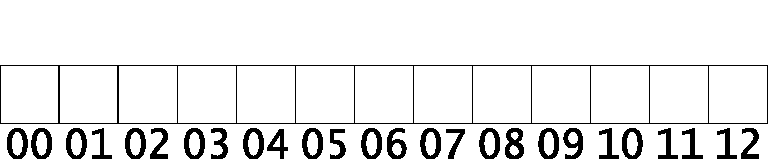
\includegraphics[width=\linewidth]{images/free}
\end{frame}

\begin{frame}[fragile]{»Dinge« und Speicher}
	Alle Definitionen legen »Dinge« an.\\
	{\tiny Ausnahme: \verb|static|}
	
	{\footnotesize
	\begin{block}{}
		\lstinputlisting[language=C++, linerange={3-4, 6-6}]{cpp-code/objects.cpp}
	\end{block}
	}
	
	\pause
	\vspace{1em}
	
	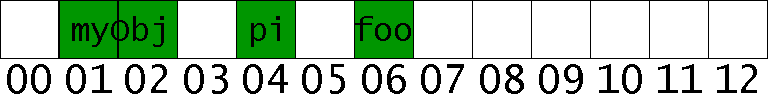
\includegraphics[width=\linewidth]{images/object_things}
\end{frame}

\begin{frame}[fragile]{»Dinge« und Referenzen}
	Eine Referenz ist ein zusätzlicher Namen für \emph{dasselbe} »Ding«.
	
	{\footnotesize
	\begin{block}{}
		\lstinputlisting[language=C++, linerange=14-15]{cpp-code/objects.cpp}
	\end{block}
	}
	
	\pause
	\vspace{1em}
	
	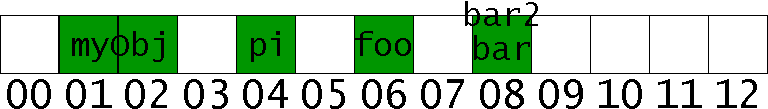
\includegraphics[width=\linewidth]{images/object_refs}
\end{frame}

\begin{frame}[fragile]{Referenzen als Parameter}
	Nutzt man eine Referenz als Parameter, so kann man innerhalb der Funktion den Wert des übergebenen »Dings« ändern:
	
	{\footnotesize
	\begin{block}{}
		\lstinputlisting[language=C++, linerange=28-32]{cpp-code/objects.cpp}
	\end{block}
	}
	
	\pause
	
	{\footnotesize
	\begin{block}{}
		\lstinputlisting[language=C++, linerange=19-22]{cpp-code/objects.cpp}
	\end{block}
	}
\end{frame}

\begin{frame}[fragile]{Adressen und Pointer}
	Jedes Byte hat eine eindeutige Adresse.
	
	Man darf keine Annahmen darüber treffen, wie diese Adresse tatsächlich aussieht oder wie groß sie ist!
	Was man tun darf, sind Operationen mit \emph{Pointern}.
	
	\pause
	
	Wir wollen jedoch zwecks Anschauung eine Adresse mit der Nummer \emph{der} Bytes eines »Dings« identifizieren.
	
	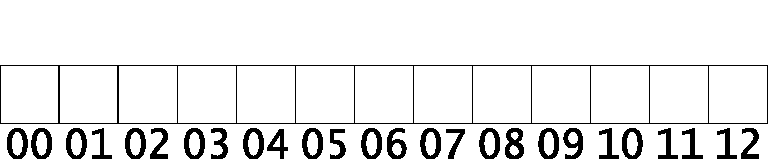
\includegraphics[width=\linewidth]{images/free}
\end{frame}

\begin{frame}[fragile]{»Dinge« und Pointer}
	Sei \verb|NAME| der Name eines »Dings«. Mit \verb|&NAME| erhalte ich dann die Adresse des »Dings«. Die Adresse selbst ist auch wieder ein »Ding«!
	
	\vspace{1em}
	\pause
	
	Als »Ding« hat die Adresse einen Typ:
	{\footnotesize
	\begin{block}{}
		\lstinputlisting[language=C++, linerange=24-25]{cpp-code/objects.cpp}
	\end{block}
	}
	
	\pause
	
	Das »Ding« \verb|NAME| habe den Typen \verb|TYPE|. Dann hat die Adresse des »Dings« den Typ \verb|TYPE*|.
\end{frame}

\begin{frame}[fragile]{»Dinge«, Pointer und Adressen}
	Ein Beispiel:
	
	{\footnotesize
	\begin{block}{}
		\lstinputlisting[language=C++, linerange={3-4, 6-6, 10-10, 27-27}]{cpp-code/objects.cpp}
	\end{block}
	}
	
	\pause
	\vspace{1em}
	
	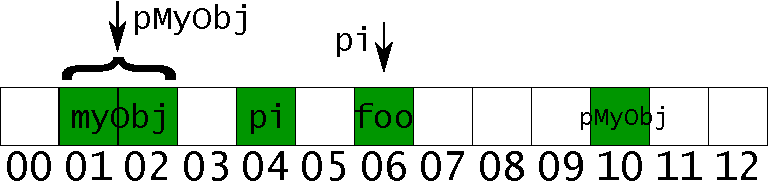
\includegraphics[width=\linewidth]{images/object_points_addr}
\end{frame}

\begin{frame}[fragile]{Pointer vs. Referenzen}
	\footnotesize
	\begin{tabular}{c|c}
		Pointer & Referenz \\ \hline
		ist ein »Ding« & ist nur ein zusätzlicher Name \\
		enthält eine Adresse & enthält selbst nichts \\
		Inhalt kann sich ändern & bezieht sich immer auf dasselbe »Ding« \\
		Inhalt muss nicht sinnvoll sein & bezieht sich auf ein existierendes »Ding« \\
	\end{tabular}
	
	\pause
	
	{\footnotesize
	\begin{block}{}
		\lstinputlisting[language=C++, linerange={4-4, 27-31}]{cpp-code/objects.cpp}
	\end{block}
	}
\end{frame}
